Any second degree equation of the form:
\begin{align}
  ax^2 + 2bxy + cy^2 + 2dx + 2ey + f = 0
\end{align}
Can be represented in matrix / vector form as:
\begin{align}
  \vec{x}^T\vec{Vx} + 2\vec{u}^T\vec{x} + f = 0
\end{align}
where,
\begin{align}
  \vec{V} = \vec{V}^T = \myvec{a & b \\ b & c} \\
  \vec{u} = \myvec{d & e}
\end{align}
Rewriting \eqref{eq:solutions/41/19/eq:1} in matrix form, we get:
\begin{align}
  \vec{x}^T\myvec{2 & \frac{3}{2} \\\frac{3}{2} & -2}\vec{x} + 2\myvec{-\frac{7}{2} & \frac{1}{2}} - 2 = 0
\end{align}
where,
\begin{align}
  \vec{V} = \myvec{2 & \frac{3}{2} \\\frac{3}{2} & -2} \\
  \vec{u} = \myvec{-\frac{7}{2} \\[0.2cm] \frac{1}{2}} \\
  f = -2 \\
  det(\vec{V}) = \mydet{2 & \frac{3}{2} \\\frac{3}{2} & -2} = -\frac{25}{4}
\end{align}
As $det(\vec{V}) < 0$, the given conic represents a hyperbola. \\
The characteristic equation of $\vec{V}$ is given by the determinant:
\begin{align}
  \mydet{\vec{V} - \lambda\vec{I}} = 0 \\
  \mydet{2 - \lambda & \frac{3}{2} \\\frac{3}{2} & -2 - \lambda} = 0 \\
  \implies \lambda^{2} - \frac{25}{4} = 0 \label{eq:solutions/41/19/eq:2}
\end{align}
The roots of \eqref{eq:solutions/41/19/eq:2} (the eigenvalues) are:
\begin{align}
  \lambda_1 = \frac{5}{2}, \lambda_2 = -\frac{5}{2}
\end{align}
The eigenvector $\vec{p}$ is defined as:
\begin{align}
  \vec{Vp} = \lambda \vec{p} \\
  \implies (\vec{V} - \lambda \vec{I})\vec{p} = 0 \label{eq:solutions/41/19/eq:3}
\end{align}
Evaluating \eqref{eq:solutions/41/19/eq:3} for $\lambda_1 = \frac{5}{2}$, we get:
\begin{align}
  (\vec{V} - \lambda_1 \vec{I})  = \myvec{-\frac{1}{2} & \frac{3}{2} \\[0.2cm]\frac{3}{2} & -\frac{9}{2}}
\end{align}
Reducing the above equation to row-echelon form, we get:
\begin{align}
  \xleftrightarrow[]{R_2 \rightarrow R_2 + 3R_1} \myvec{-\frac{1}{2} & \frac{3}{2} \\[0.2cm]0 & 0} \xleftrightarrow[]{R_1 \rightarrow -2R_1} \myvec{1 & -3 \\ 0 & 0} \label{eq:solutions/41/19/eq:4}
\end{align}
Substituting \eqref{eq:solutions/41/19/eq:4} in \eqref{eq:solutions/41/19/eq:3}, we get:
\begin{align}
  \myvec{1 & -3 \\ 0 & 0} \myvec{v_1 \\ v_2} = \myvec{0 \\ 0}
\end{align}
where,
\begin{align}
  \vec{p} = \myvec{v_1 \\ v_2}
\end{align}
Let $v_2 = t$. Then
\begin{align}
  v_1 = 3t
\end{align}
Let $t = 1$. The eigenvector $\vec{p_1}$ is:
\begin{align}
  \vec{p_1} = \myvec{3 \\ 1}
\end{align}
Similarly for $\lambda_2 = -\frac{5}{2}$, we get:
\begin{align}
    (\vec{V} - \lambda_2 \vec{I})  = \myvec{\frac{9}{2} & \frac{3}{2} \\[0.2cm]\frac{3}{2} & \frac{1}{2}} \xleftrightarrow[R_1 \rightarrow \frac{2}{9}R_1]{R_2 \rightarrow 3R_2 - R_1} \myvec{1 & \frac{1}{3} \\[0.2cm]0 & 0} \label{eq:solutions/41/19/eq:5}
\end{align}
Substituting \eqref{eq:solutions/41/19/eq:5} in \eqref{eq:solutions/41/19/eq:3}, we get:
\begin{align}
  \myvec{1 & \frac{1}{3} \\[0.2cm]0 & 0} \myvec{v_1 \\ v_2} = \myvec{0 \\ 0}
\end{align}
where,
\begin{align}
  \vec{p} = \myvec{v_1 \\ v_2}
\end{align}
Let $v_2 = t$. Then
\begin{align}
  v_1 = \frac{-t}{3}
\end{align}
Let $t = 1$. The eigenvector $\vec{p_2}$ is:
\begin{align}
  \vec{p_2} = \myvec{\frac{-1}{3} \\[0.2cm] 1}
\end{align}
As $\vec{V} = \vec{V}^T$, there exists an orthogonal matrix P such that:
\begin{align}
  \vec{PVP}^T = \vec{D} = diag(\lambda_1, \lambda_2)
\end{align}
$\vec{V}$ can be rewritten using the above equation as:
\begin{align}
  \vec{V} = \vec{PDP}^T
\end{align}
where,
\begin{align}
  \vec{P} = \myvec{\vec{p_1} & \vec{p_2}} \\
  \vec{D} = \myvec{\lambda_1 & 0 \\ 0 & \lambda_2}
\end{align}
Substituting the values -
\begin{align}
  \vec{P} = \myvec{3 & \frac{-1}{3}\\[0.2cm] 1 & 1} \\
  \vec{D} = \myvec{\frac{5}{2} & 0 \\[0.2cm] 0 & \frac{-5}{2}}
\end{align}
The center of hyperbola is given by:
\begin{align}
  \vec{c} = -\vec{V}^{-1}\vec{u} \\
  \implies \vec{c} = -\myvec{\frac{8}{25} & \frac{6}{25} \\[0.2cm] \frac{6}{25} & \frac{-8}{25}} \myvec{\frac{-7}{2} \\[0.2cm]\frac{1}{2}} = \myvec{1 \\ 1}
\end{align}
As
\begin{align}
  \vec{u}^T\vec{V}^{-1}\vec{u} - f = 5 > 0
\end{align}
there is no requirement for swapping the axes (which will be evident from the equation below). The axes of the hyperbola are given by:
\begin{align}
  axes = \begin{cases}
    \sqrt[]{\frac{\vec{u}^T\vec{V}^{-1}\vec{u} - f}{\lambda_1}} \\
    \sqrt[]{\frac{f - \vec{u}^T\vec{V}^{-1}\vec{u}}{\lambda_2}}
  \end{cases} \\
  \implies \sqrt[]{\frac{\vec{u}^T\vec{V}^{-1}\vec{u} - f}{\lambda_1}} = \sqrt[]{2} \\
  \implies \sqrt[]{\frac{f - \vec{u}^T\vec{V}^{-1}\vec{u}}{\lambda_2}} = \sqrt[]{2}
\end{align}
The standard form of conic is written as:
\begin{align}
  \vec{y}^T\vec{Dy} = \vec{u}^T\vec{V}^{-1}\vec{u} - f
\end{align}
where,
\begin{align}
  \vec{y} = \vec{P}^T(\vec{x-c}) \\
  \implies \vec{y}^T \myvec{\frac{5}{2} & 0 \\[0.2cm] 0 & \frac{-5}{2}} \vec{y} -5 = 0
\end{align}
The plot of both the conics are given below:
\begin{figure}[h!]
\centering
    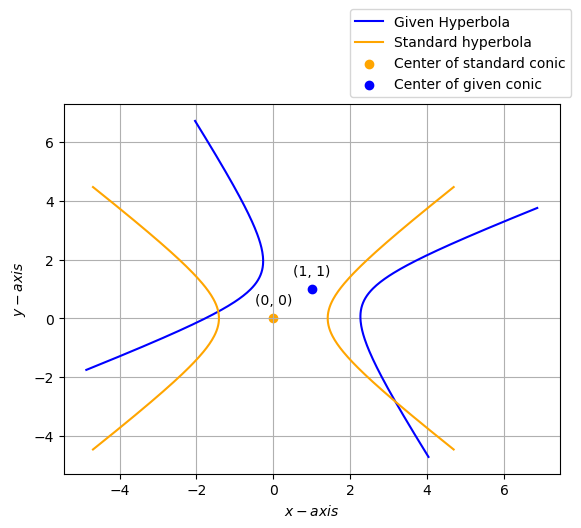
\includegraphics[width=\columnwidth]{solutions/41/19/Latex/hyperbola.png}
    \caption{Plot of given hyperbola and the standard hyperbola}
    \label{eq:solutions/41/19/fig:1}
\end{figure}
